\section{Performance Evaluation}
\label{sec:evaluation}
In this section, we evaluate the performance of the proposed low-complexity dispatching policy $\tilde{\Policy}$ by numerical simulations.
The experiment setup and performance benchmarks are described in Section \ref{subsec:setup}.
We give the simulation results in Section \ref{subsec:basic}.
The sensitivity study on parameters is also applied which provides some insights on the robustness of the proposed policy, as discussed in Section \ref{subsec:advance}.

\subsection{Experiment Setup}
\label{subsec:setup}
In the simulation, we assume that there are $K=15$ APs, $M=10$ edge servers and $J=10$ types of jobs in the system.
One broadcast interval consists of $t_{B}=25$ time slots.
The network topology is generated according to the Barab\'asi-Albert (BA) model \cite{albert1999diameter}.
The edge servers are randomly placed and collocated with the APs.
The arrival traces and job processing time for each job type are extracted from the Google cluster traces \cite{clusterdata:Reiss2011} and then randomly assigned to the APs and edge servers, respectively.
The maximum uploading latency is $\Xi = 3t_B$, and the distribution of $\mathbb{U}_{k,m,j}(\Xi)$ ($\forall k\in\apSet, m\in\esSet_{k}, j\in\jSpace$) is arbitrarily generated within the support $\set{0, 1, \dots, \Xi}$.
The \brlatency~is with an integer support from $0.7t_B$ to $0.9t_B$ time slots.
Each queue for VM on an edge server is with maximum queue length $L_{max}=50$, i.e., there would be at most $50$ jobs on any edge server.
The discount factor $\gamma$ is $0.95$ and the overflow penalty weight $\beta$ is $120$.

%-----------------------------------------------------------------------%
\begin{figure}[ht]                                                      %
    \centering                                                          %
    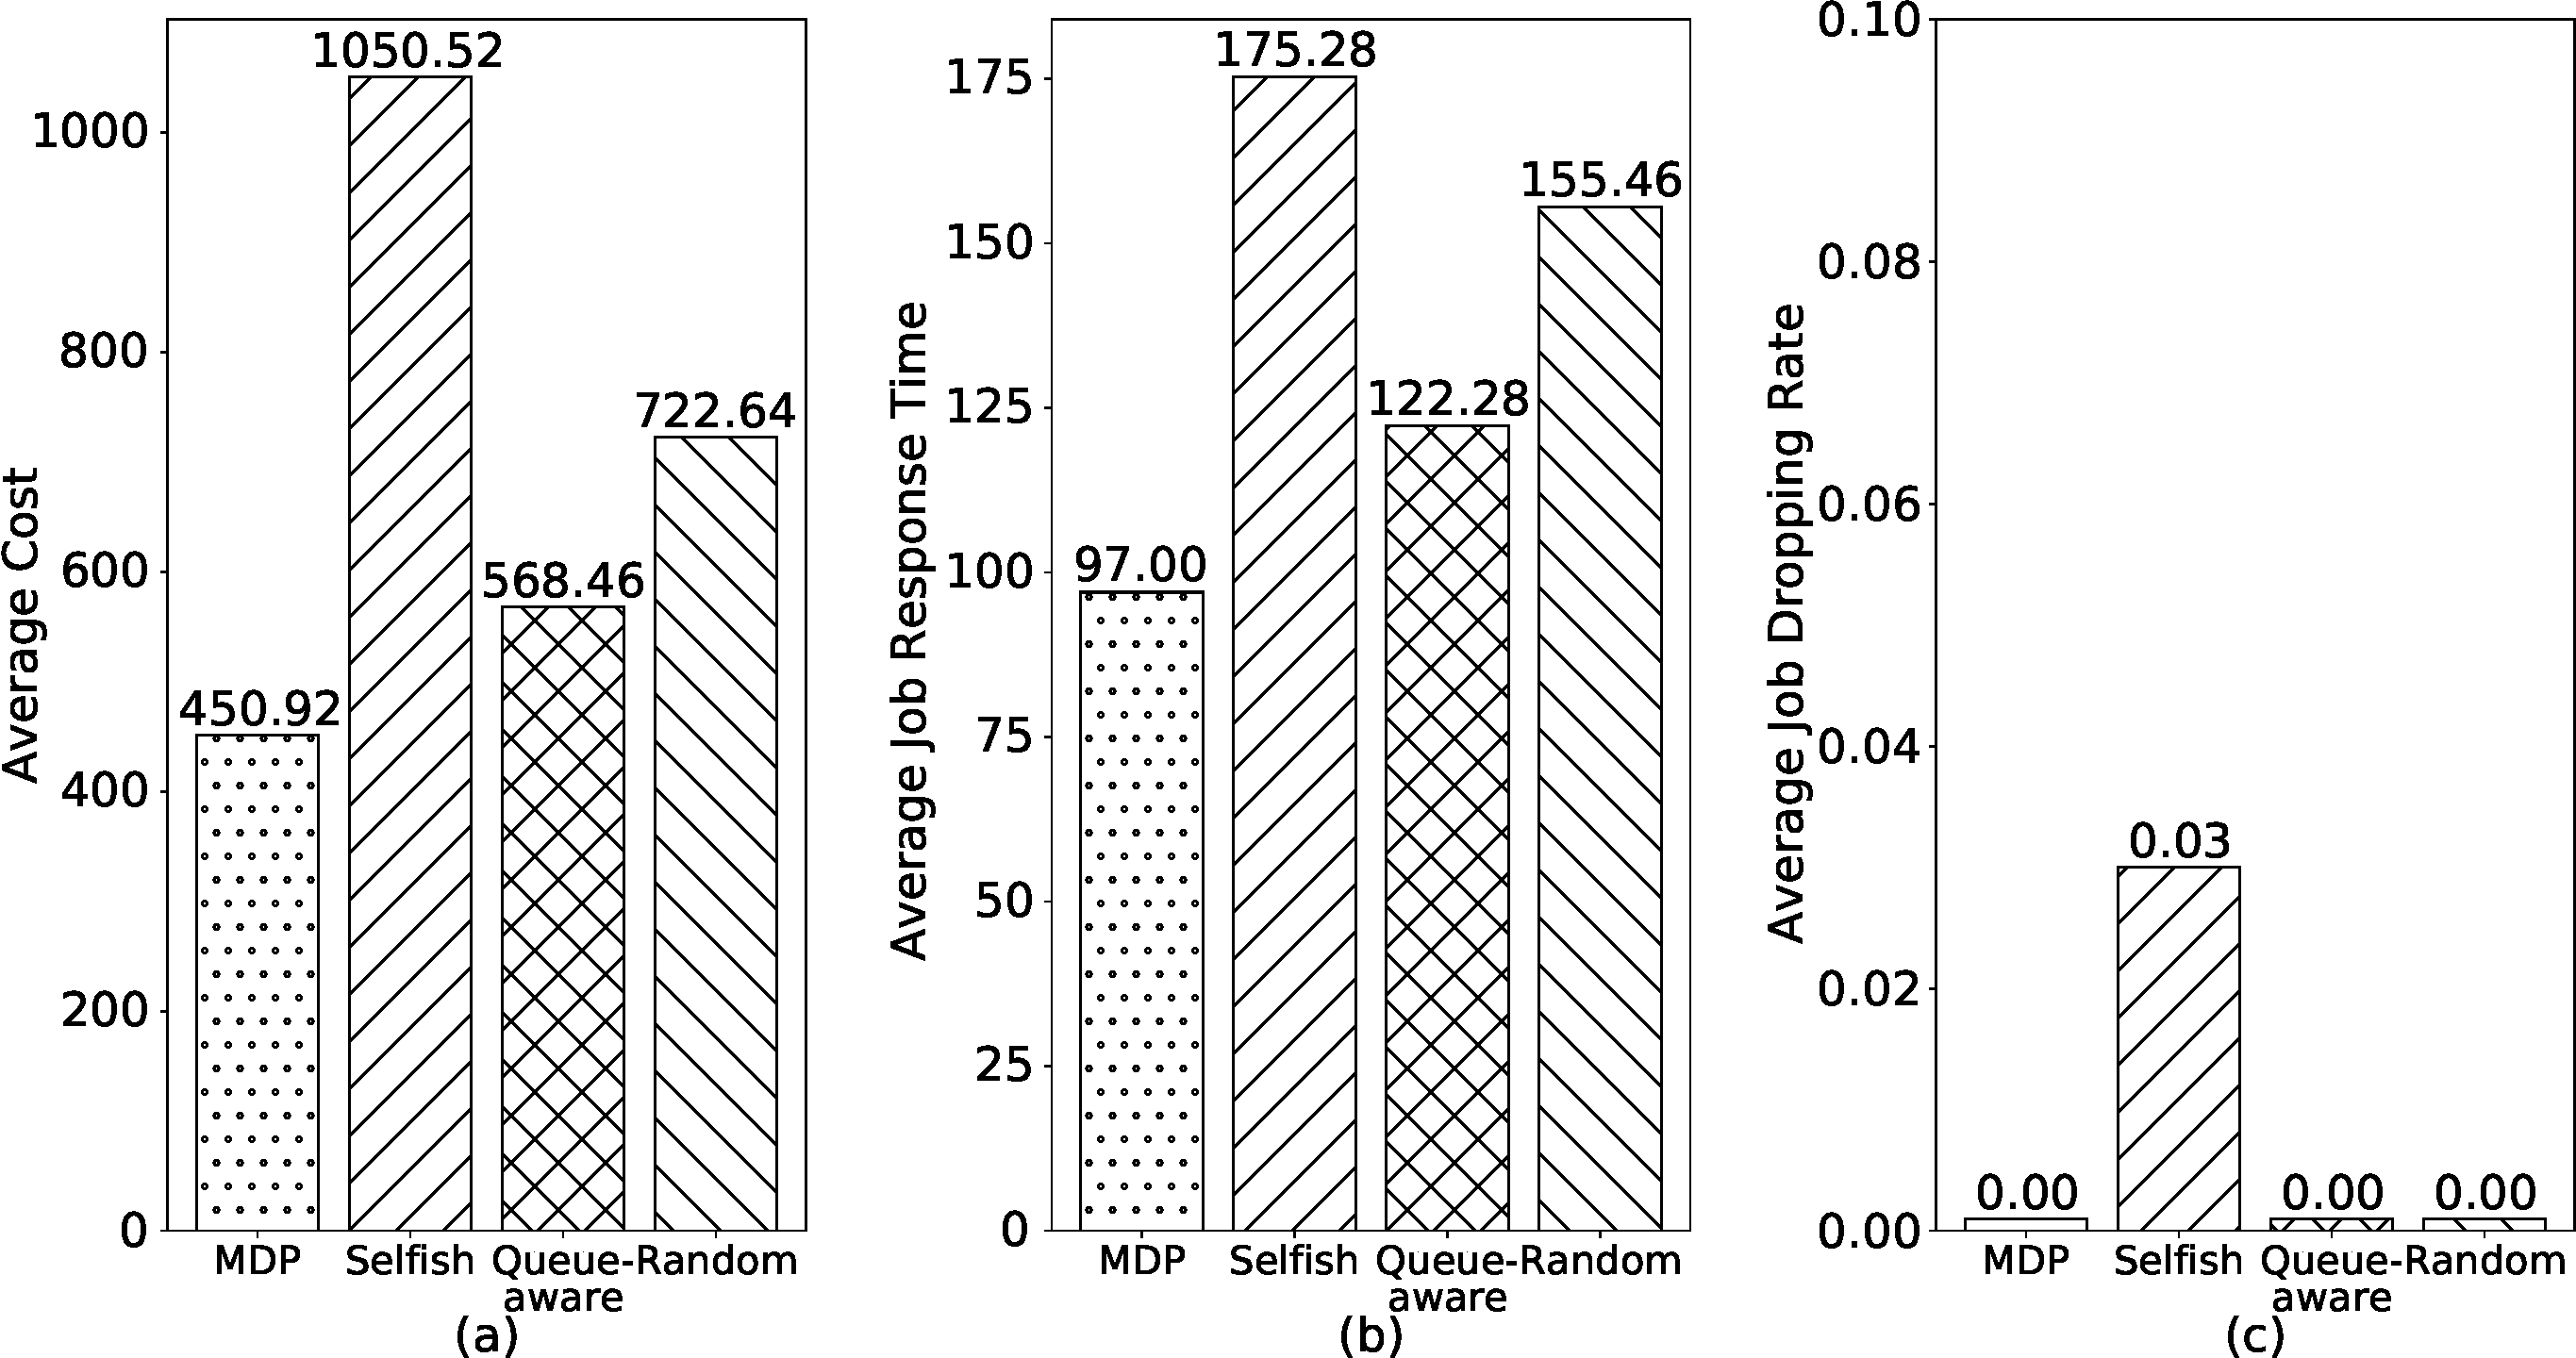
\includegraphics[width=0.45\textwidth]{hong5.pdf}               %
    \caption{Performance comparison with benchmarks.}
    \label{fig:bar_plot}                                                %
\end{figure}                                                            %
%-----------------------------------------------------------------------%

We also propose {three heuristic benchmarks to profile the performance of the proposed solution framework \algname}:
\begin{itemize}
    \item \textbf{Random Policy}:
            Randomly choose a dispatching edge server in each time slot; 
    \item \textbf{Selfish Policy}:
            Always choose the edge server with the minimum sum of the expected uploading time and processing time;
    \item \textbf{Queue-aware Policy}:
            Always choose the edge server with the minimum sum of expected uploading time, processing time and queueing time based on the observation of outdated queue status.
\end{itemize}
Moreover, we choose the Selfish Policy as the initial dispatching action (Baseline Policy) for our proposed algorithm (Algorithm \ref{alg_1}).

\subsection{Performance Analysis}
\label{subsec:basic}
As illustrated in Fig.~\ref{fig:bar_plot}(a), the proposed policy (MDP Policy) outperforms all the benchmarks in terms of average system cost.
More insights on the performance comparison are provided in Fig.~\ref{fig:bar_plot}(b) and (c).
In the former figure, the average job response times, measuring the average number of broadcast intervals from job's arrival at one AP to the completeness of computation at one edge server, are compared.
It can be observed that the proposed policy still outperforms all the benchmarks.
In Fig.~\ref{fig:bar_plot}(c), the job dropping rates, measuring the ratio of jobs dropped by edge servers due to queue overflow, are also compared.
{In} summary, the proposed policy outperforms {the} other three benchmarks in terms of minimum average cost and job response time.
Moreover, the proposed policy has no dropping jobs although the Selfish policy is used as the initial baseline policy for our algorithm.
Finally, a running trace of job dispatching is shown in Fig.~\ref{fig:general_timeline}, where the \hongyc{cost (number of jobs plus the overflow penalty) raised in the system} is plotted against the index of broadcast interval.
Clearly, the proposed policy manages to keep the number of jobs at a lower level, as compared with the other benchmarks.
This demonstrates its high dispatching efficiency.

In Fig.~\ref{fig:semi-bound}, the simulation result demonstrates the vanishing gap between the semi-analytical cost upper bound $W^{(T)}_{\hat{\Baseline}}(\Stat)$ and the actual average performance of the proposed policy for different $T$s.
It shows that the proposed policy $\tilde{\Policy}$ is bounded and the performance gap $e(T)$ decreases monotonically when $T$ increases, yielding a trade-off between evaluation accuracy and computation complexity.

%-----------------------------------------------------------------------------------------------%
\begin{figure}[ht!]                                                                             %
    \centering                                                                                  %
    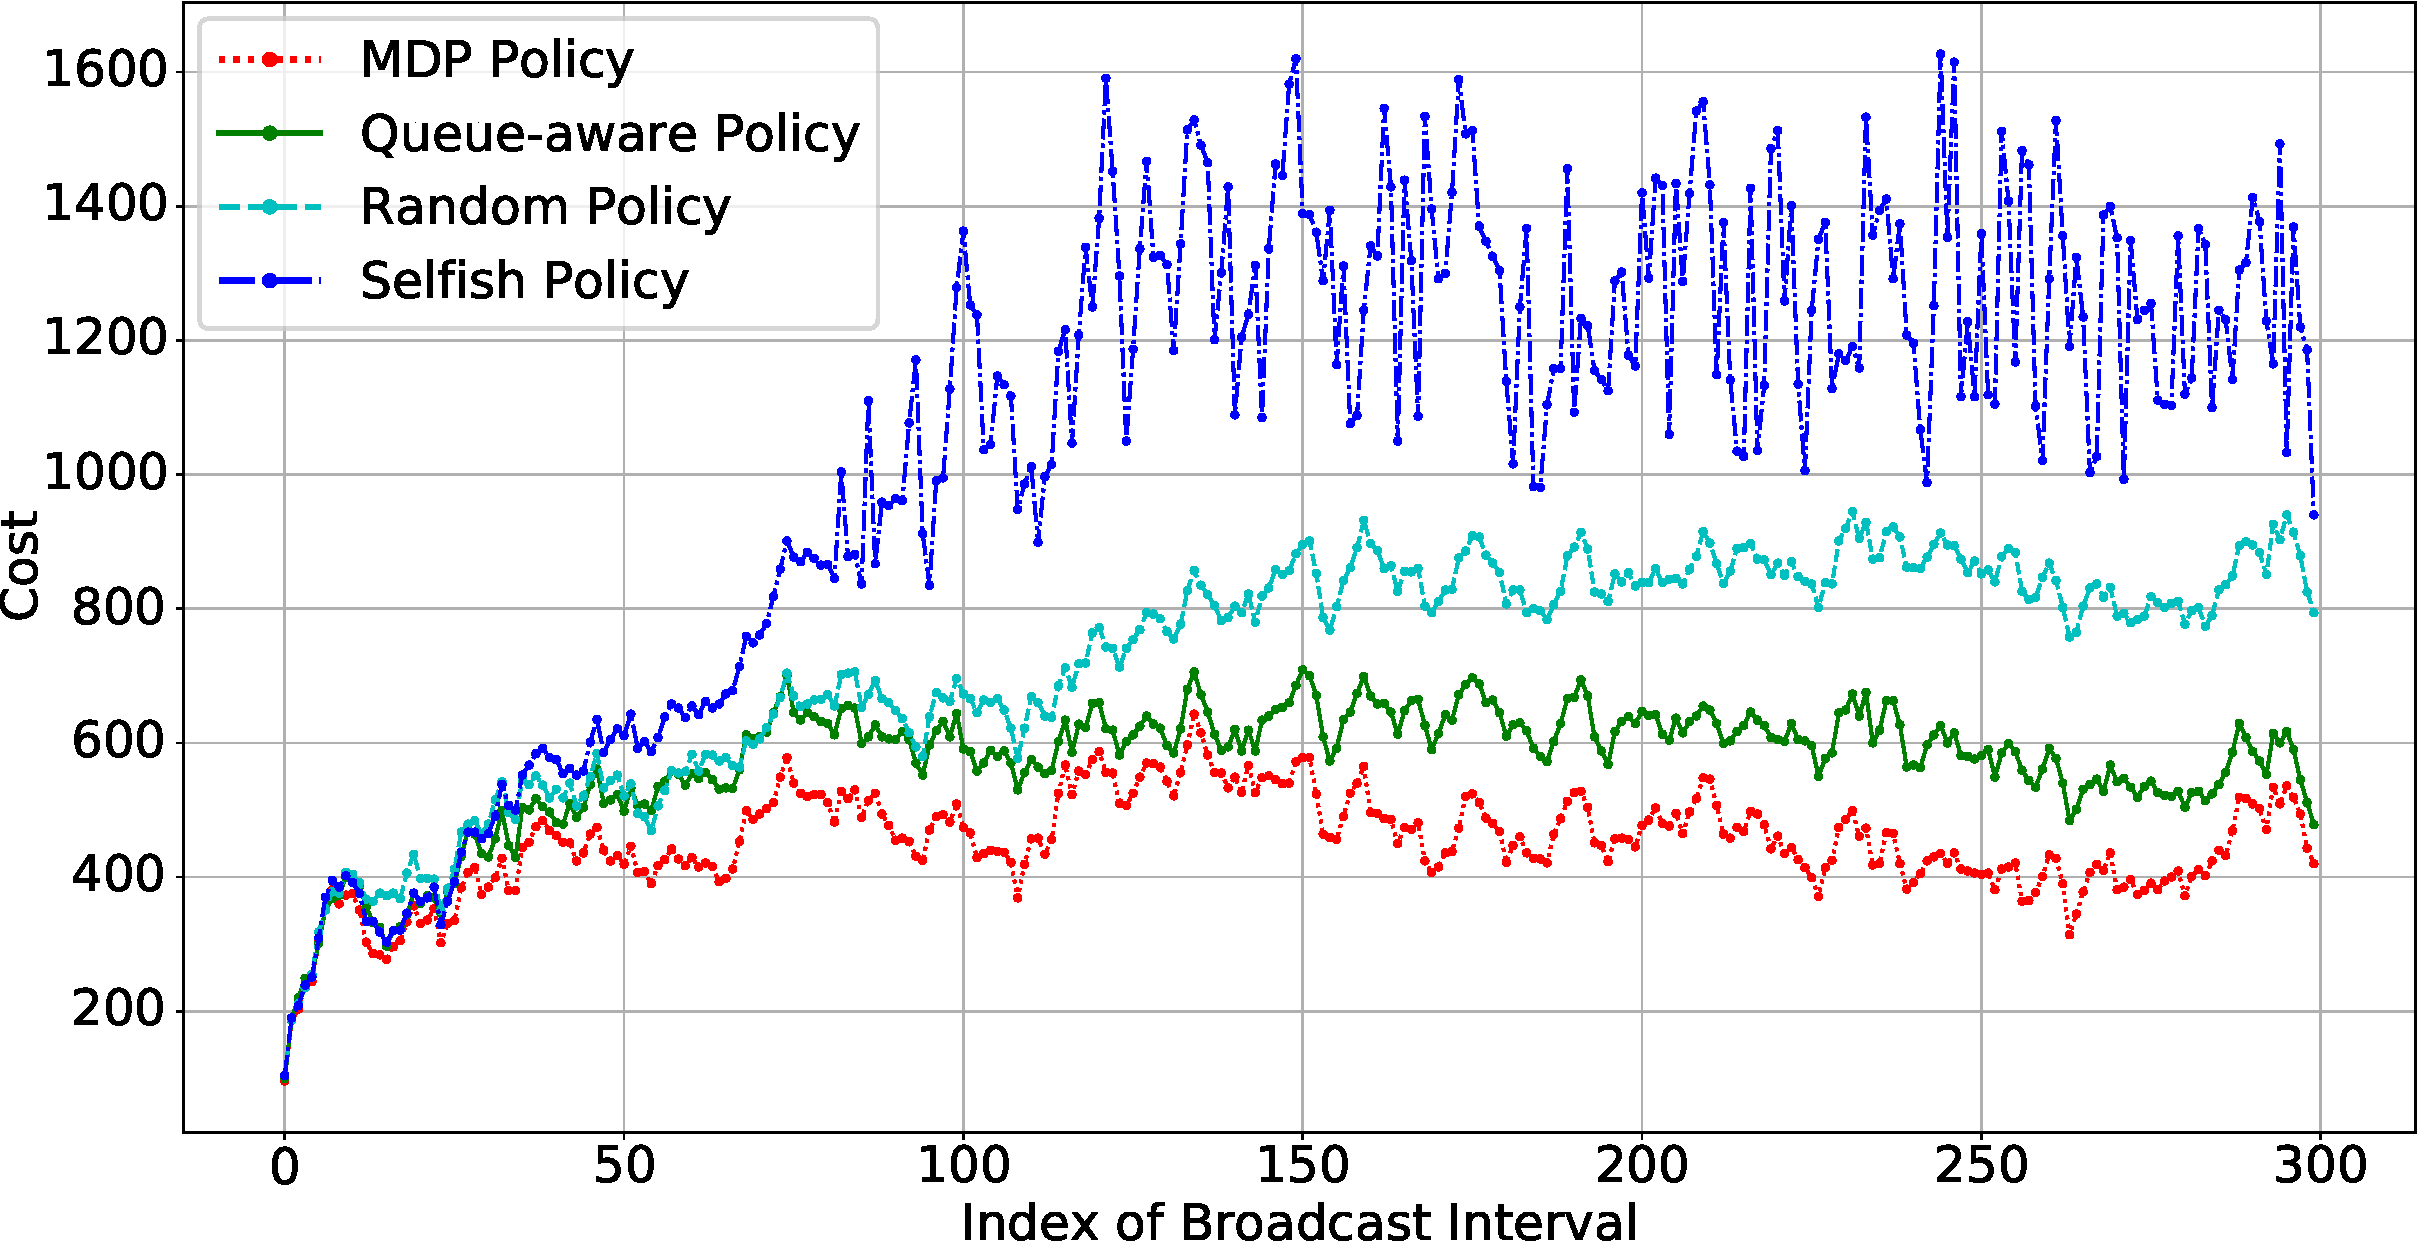
\includegraphics[width=0.45\textwidth]{hong6.pdf}                     %
    \caption{Costs versus over the broadcast intervals.}
    \label{fig:general_timeline}                                                                %
\end{figure}                                                                                    %
%-----------------------------------------------------------------------------------------------%

%-----------------------------------------------------------------------------------------------%
\begin{figure}[ht!]                                                                             %
    \centering                                                                                  %
    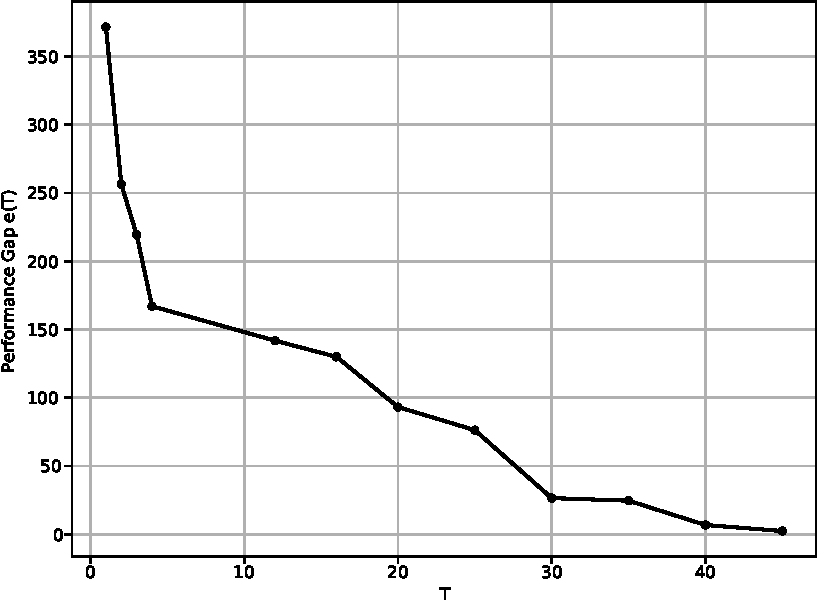
\includegraphics[width=0.45\textwidth]{hong7.pdf}                     %
    \caption{The performance gap between $W^{(T)}_{\hat{\Baseline}}(\Stat)$ and $W_{\tilde{\Policy}}(\Stat)$ versus the stage number of numerical evaluation T.}
    \label{fig:semi-bound}                                                                %
\end{figure}                                                                                    %
%-----------------------------------------------------------------------------------------------%

\subsection{Convergence Analysis}
\label{subsec:converge}
The convergence property of the proposed reinforcement learning algorithm is illustrated in Fig.~\ref{fig:rl_plot}.
It can be observed that the learning procedures for all the three statistical parameters converge after $80$ broadcast intervals.
In comparison, the number of observations required for the convergence of conventional reinforcement learning algorithms is usually much larger for enormous system and action spaces.
This demonstrates the efficiency of the proposed reinforcement learning algorithm, which benefits from the derived expression {of} the approximate value function.
\begin{figure}[ht!]
    \centering
    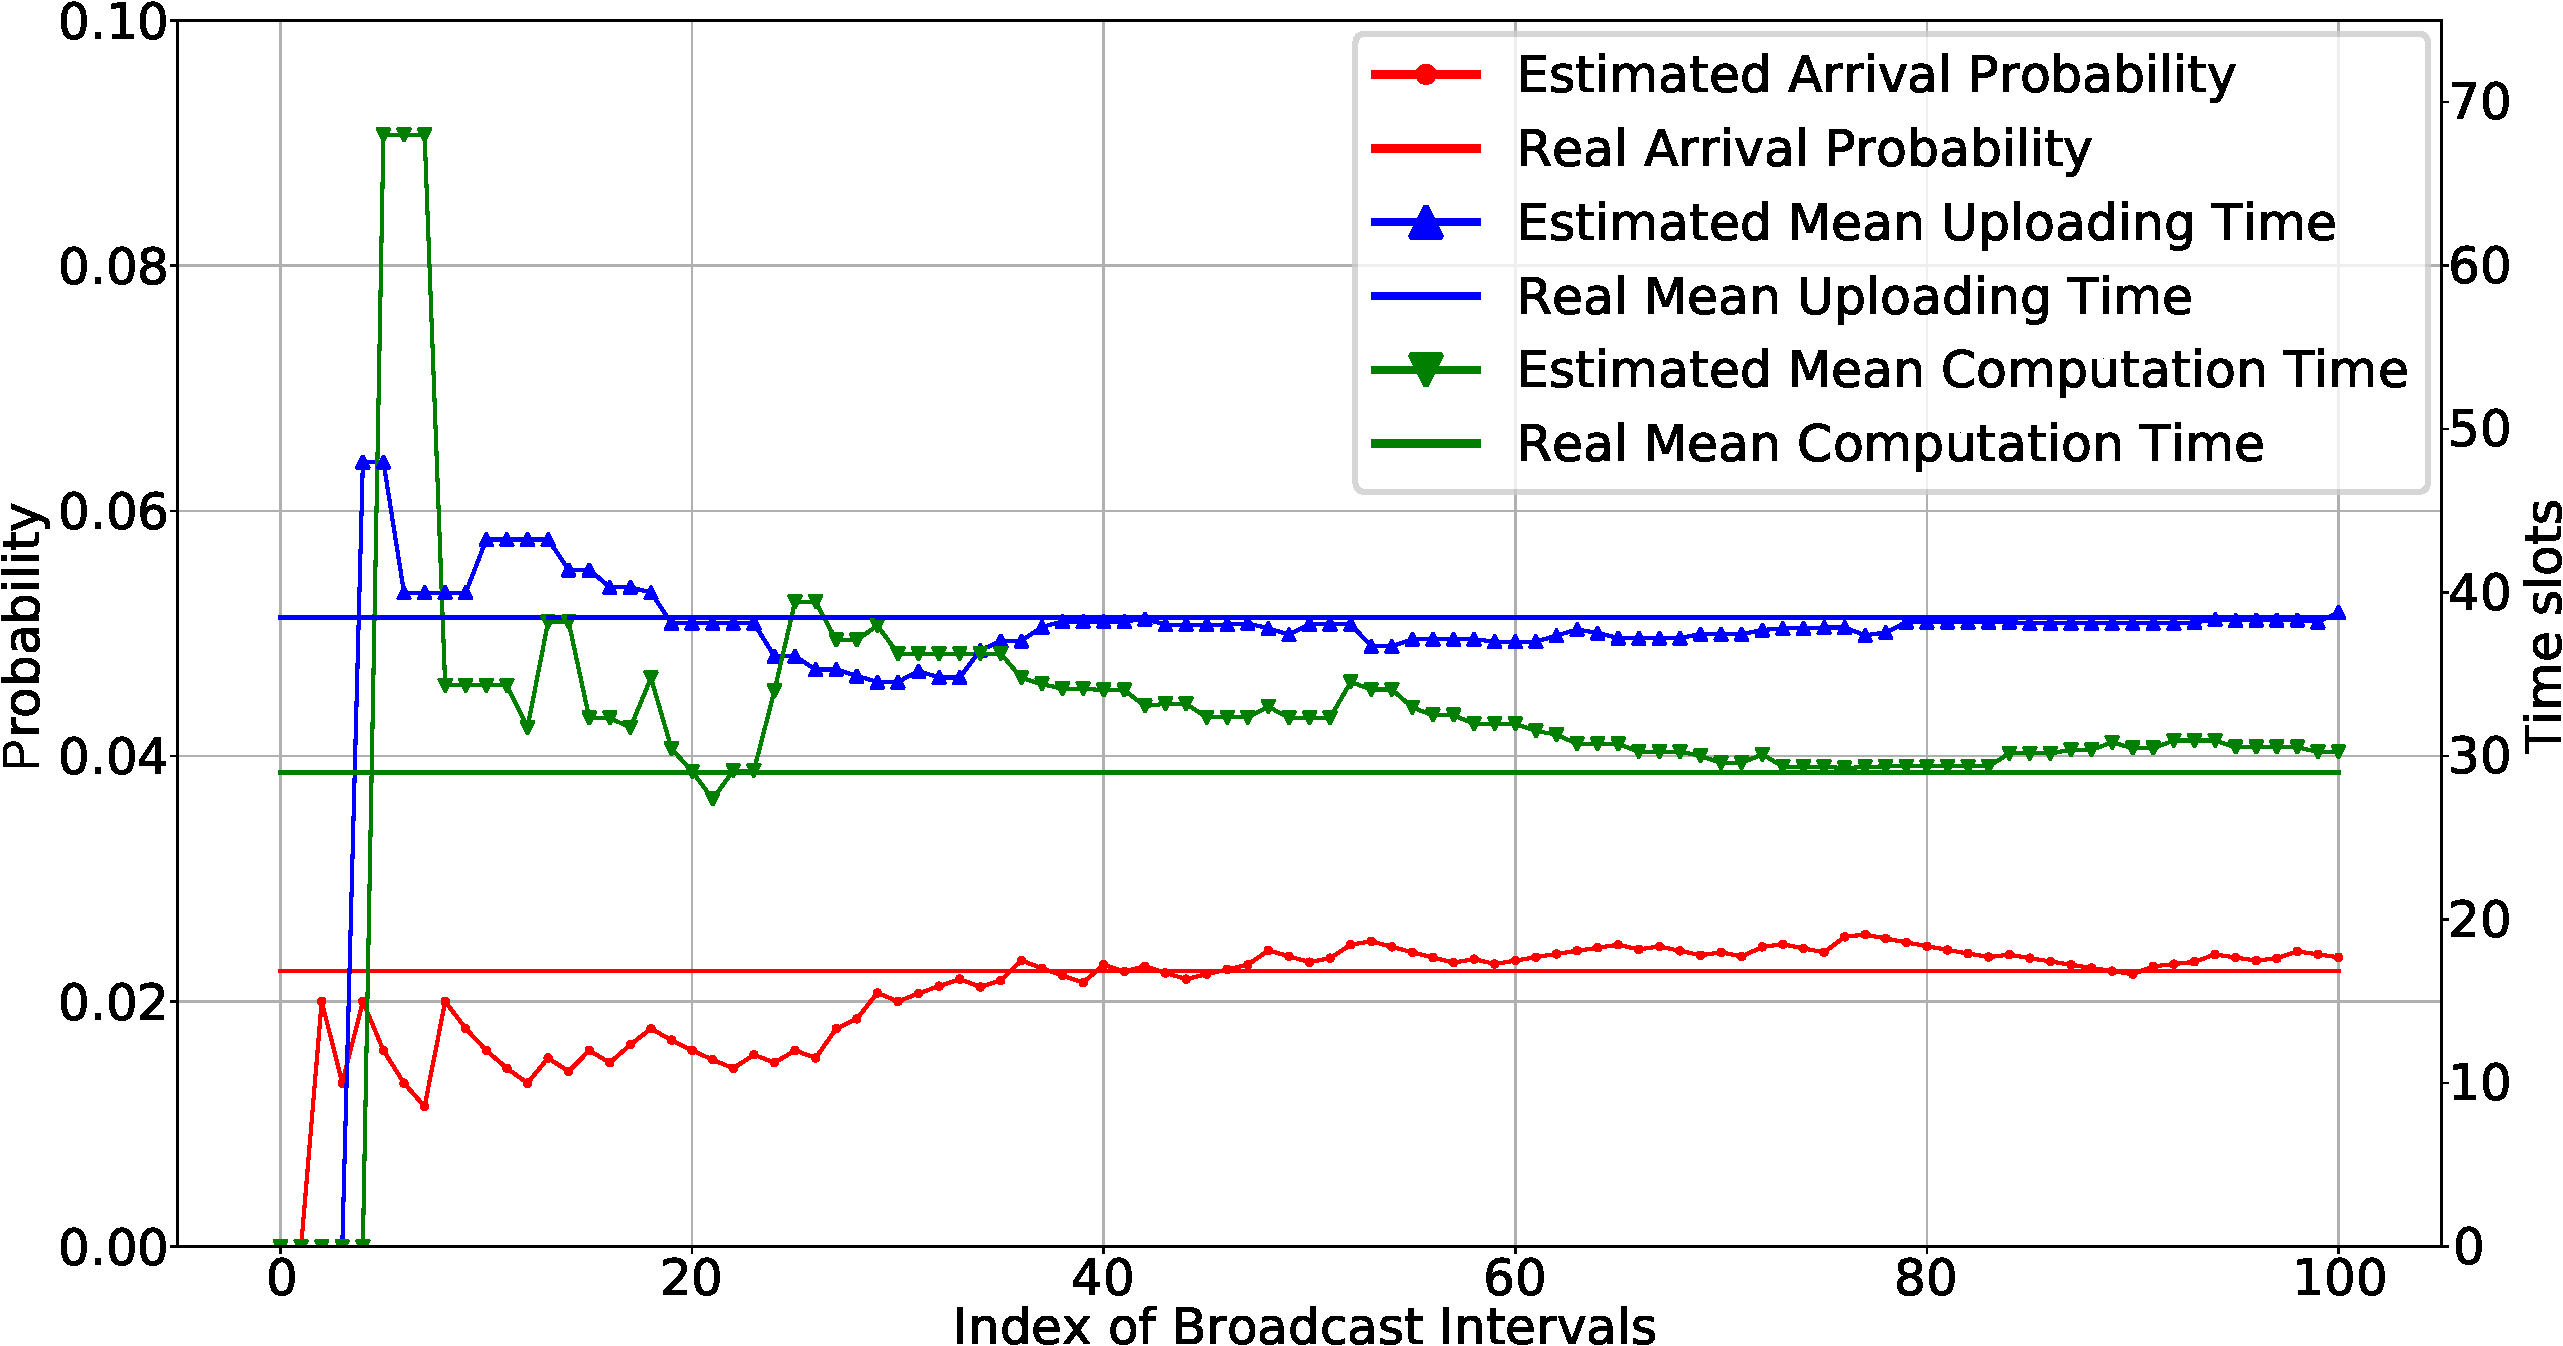
\includegraphics[width=0.45\textwidth]{hong8.pdf}
    \caption{Convergence of the reinforcement learning algorithm.} 
    \label{fig:rl_plot}
\end{figure}

\subsection{Sensitivity Study}
\label{subsec:advance}
%-----------------------------------------------------------------------------------%
\begin{figure*}[ht!]                                                                %
    \centering                                                                      %
    \begin{minipage}[b]{0.30\textwidth}                                             %
        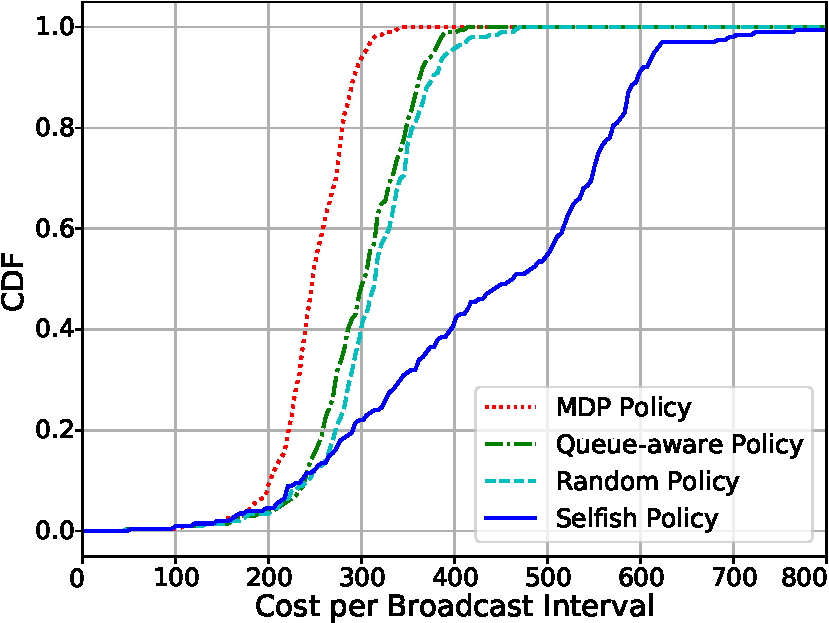
\includegraphics[width=\textwidth]{hong9.pdf} \\              %
        (a) Latency = $5$ time slots
    \end{minipage}                                                                  %
    \begin{minipage}[b]{0.30\textwidth}                                             %
        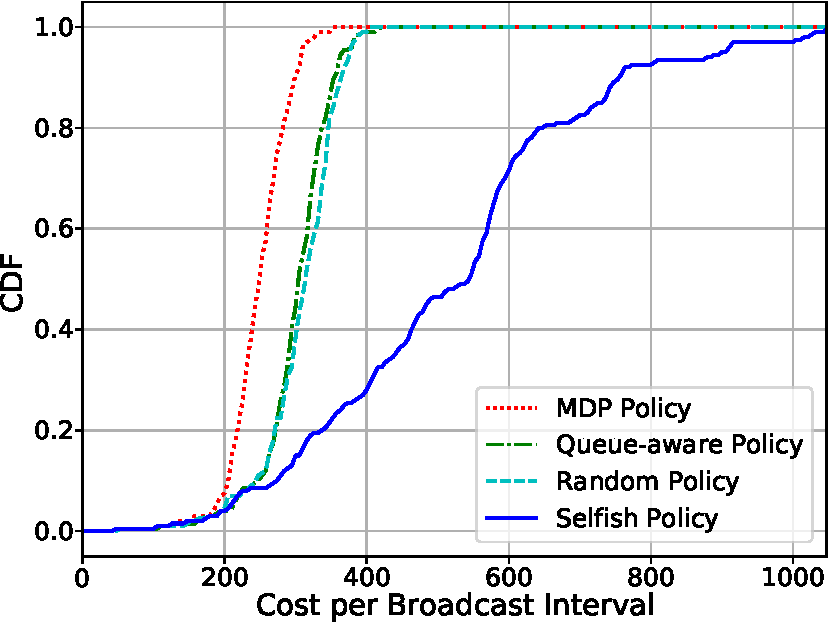
\includegraphics[width=\textwidth]{hong10.pdf} \\             %
        (b) Latency = $12$ time slots
    \end{minipage}                                                                  %
    \begin{minipage}[b]{0.30\textwidth}                                             %
        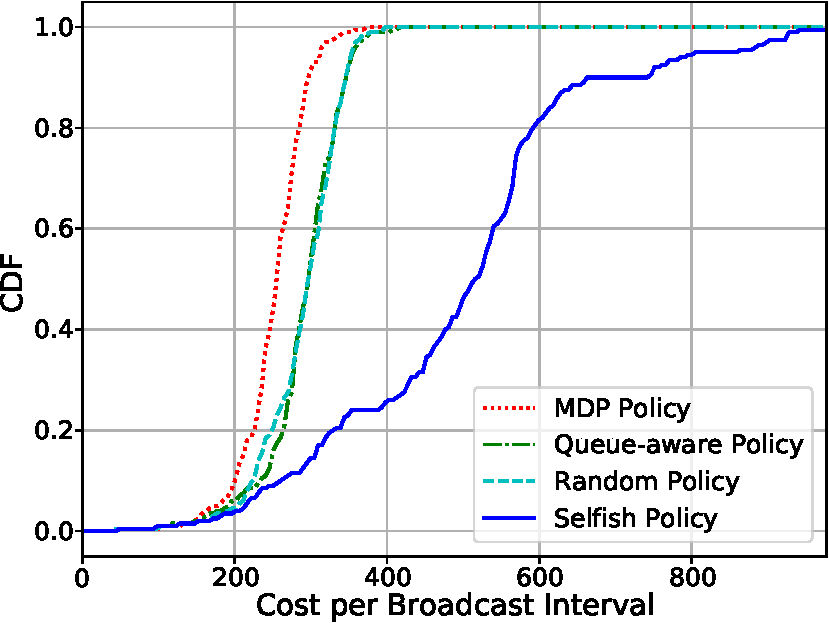
\includegraphics[width=\textwidth]{hong11.pdf} \\               %
        (c) Latency = $25$ time slots
    \end{minipage}                                                                  %
    \caption{Algorithm robustness versus various signaling latencies.}                %
    \label{fig:ss_signal}                                                           %
\end{figure*}                                                                       %
%-----------------------------------------------------------------------------------%


%-------------------------------------------------------------------%
\begin{figure}[hbt]                                                 %
    \centering                                                      %
    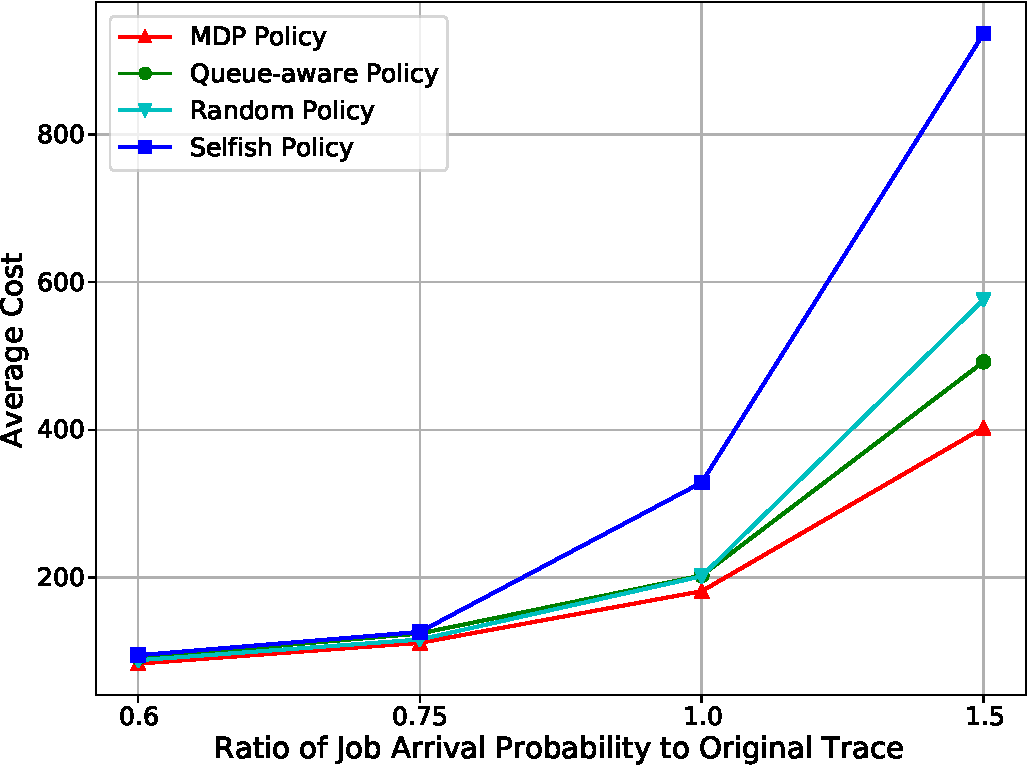
\includegraphics[width=0.45\textwidth]{hong12.pdf}   %
    \caption{Average system cost versus job arrival intensity.}
    \label{fig:ss_scale}                                            %
\end{figure}                                                        %
%-------------------------------------------------------------------%

%-------------------------------------------------------------------%
\begin{figure}[hbt]                                                 %
    \centering                                                      %
    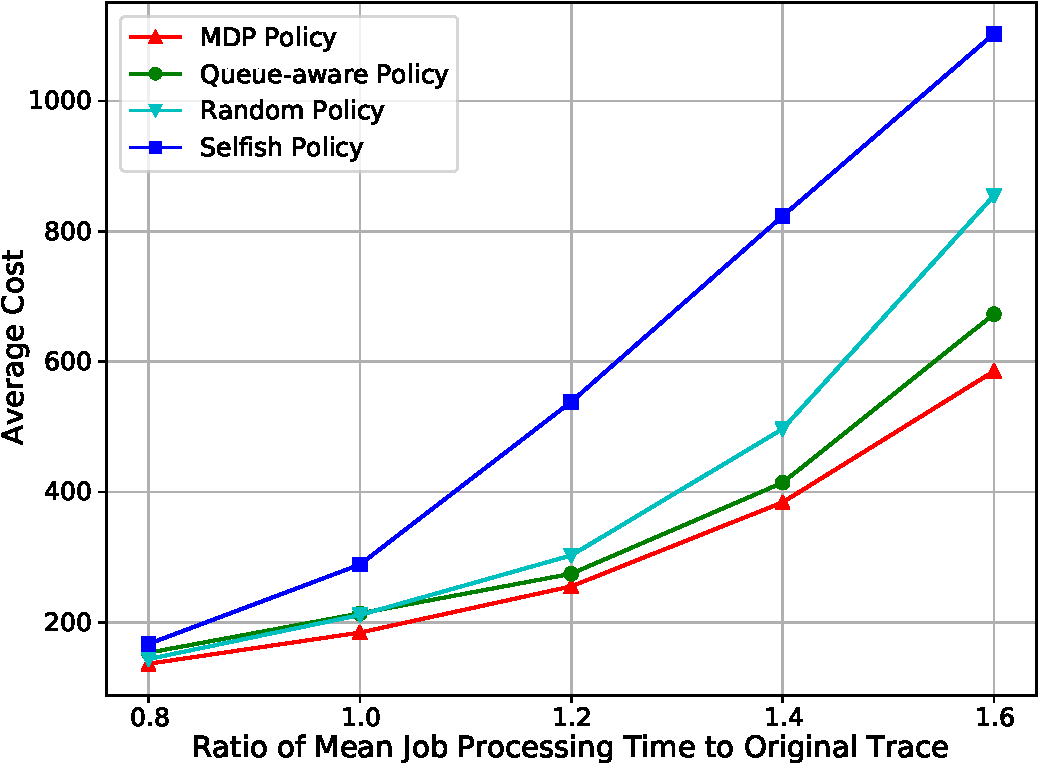
\includegraphics[width=0.45\textwidth]{hong13.pdf}      %
    \caption{Average system cost versus mean processing time.}
    \label{fig:ss_dist}                                             %
\end{figure}                                                        %
%-------------------------------------------------------------------%

\noindent\textbf{Signaling Latency.}
The simulation results with different \brlatency~$\mathcal{D}_{k}$ ($\forall k\in\apSet$) are illustrated in Fig.~\ref{fig:ss_signal}, where the cumulative distribution function (CDF) of the job number in the system is plotted.
Specifically, the \brlatency~of all the APs is set to $5, 12, 25$ in Fig.~\ref{fig:ss_signal}(a), Fig.~\ref{fig:ss_signal}(b), and Fig.~\ref{fig:ss_signal}(c), respectively.
It can be observed from Fig.~\ref{fig:ss_signal}(a) to Fig.~\ref{fig:ss_signal}(c) that, with the increasing of \brlatency, the performance of Queue-aware Policy becomes worse.
The Queue-aware policy slightly outperforms the Random Policy in Fig.~5(a) with smaller \brlatency~(achieving a smaller number of jobs in the system), and becomes worse in Fig.~5(c) with large \brlatency.
This demonstrates that the Queue-aware Policy is sensitive to the \brlatency.
In all the figures, the proposed policy outperforms all the benchmarks, which confirms its robustness against signaling latency.

\noindent\textbf{Job Arrival Probability.}
We carry out the sensitivity study of job arrival probability by scaling the interval of jobs arriving in the Google cluster traces.
% The simulation results of various arrival probability are illustrated in Fig.\ref{fig:ss_scale}.
The average system cost versus the number of APs is shown in Fig.~\ref{fig:ss_scale}.
With the {increase} of job arrival probability, the average system cost increases in all the benchmarks as well as our proposed policy.
It can be observed that our policy performs the best.
Moreover, the performance gain becomes significant when the computation load is heavy.
This speaks for the dispatching efficiency of the proposed policy with heavy load.
The gain is negligible for light load, where the computation capability is sufficient and dispatcher optimization may not be necessary.

\noindent\textbf{Mean Processing Time.}
The simulation results with different mean processing times $\set{c_{m,j}|\forall m\in\esSet,j\in\jSpace}$ are illustrated in Fig.~\ref{fig:ss_dist}, where the average processing time from the Google cluster traces is scaled by a factor from $0.8$ to $1.6$ respectively.
%in our computation model assumption.
Generally, with the increasing average processing time, the average system cost increases in all the benchmarks and our proposed policy.
The simulation results are consistent with those in Fig.~\ref{fig:ss_scale}.
It can be easily seen that the proposed policy has better performance than the benchmarks.
Moreover, the performance gain becomes significant when the computation time is long.
%----------------------------------------------------------------------------------------%